\documentclass[12pt]{article}

\usepackage[hidelinks]{hyperref}
\usepackage{graphicx}
\usepackage{color}
\usepackage{xcolor}
\usepackage{listings}
\usepackage{courier}
\usepackage{amsmath}

% syntax highlighting from: http://www.kv0.org/blog/2010/12/15/vernunftiges-syntax-highlighting-in-latex/
\lstset{
	basicstyle=\footnotesize\ttfamily, % Standardschrift
	numbers=left, % Ort der Zeilennummern
	numberstyle=\tiny, % Stil der Zeilennummern
	%stepnumber=2, % Abstand zwischen den Zeilennummern
	numbersep=5pt, % Abstand der Nummern zum Text
	tabsize=2, % Groesse von Tabs
	extendedchars=true, %
	breaklines=true, % Zeilen werden Umgebrochen
	keywordstyle=\color{orange}\bfseries,
	frame=b,
	% keywordstyle=[1]\textbf, % Stil der Keywords
	% keywordstyle=[2]\textbf, %
	% keywordstyle=[3]\textbf, %
	% keywordstyle=[4]\textbf, \sqrt{\sqrt{}} %
	stringstyle=\color{white}\ttfamily, % Farbe der String
	showspaces=false, % Leerzeichen anzeigen ?
	showtabs=false, % Tabs anzeigen ?
	xleftmargin=17pt,
	framexleftmargin=17pt,
	framexrightmargin=5pt,
	framexbottommargin=4pt,
	commentstyle=\color{green},
	% backgroundcolor=\color{gray},
	showstringspaces=false, % Leerzeichen in Strings anzeigen ?
	morekeywords={__global__} % CUDA specific keywords
}
\lstloadlanguages{% Check Dokumentation for further languages ...
%[Visual]Basic
%Pascal
C,
C++,
%XML
%HTML
Java
}
%\DeclareCaptionFont{blue}{\color{blue}}
 
%\captionsetup[lstlisting]{singlelinecheck=false, labelfont={blue}, textfont={blue}}
\usepackage{caption}
\DeclareCaptionFont{white}{\color{white}}
\DeclareCaptionFormat{listing}{\colorbox{gray}{\parbox{\textwidth}{\hspace{15pt}#1#2#3}}}
\captionsetup[lstlisting]{format=listing,labelfont=white,textfont=white, singlelinecheck=false, margin=0pt, font={bf,footnotesize}}

\title{Project Report - Second assignment - GAME ENGINES}
\author{Andrea Distler}
\date{05 December, 2012}

\begin{document}
\maketitle
\newpage

\tableofcontents
\newpage

%------------------------------------------
\section{Introduction}
This is the project report for the second assignment of the Game Engines course.

A short description of the source code and the used libraries can be found in section \ref{section:files}. The files are available on GitHub. The libraries are also made available on GitHub for easier installation.

In section \ref{section:outcome} the outcome is described. In section \ref{section:classes} used mechanics and an overview of the classes can be found.

%------------------------------------------
\section{The Files}
\label{section:files}
All files can be found on GitHub. \newline 
\url{https://github.com/JungleJinn/GE---SimplePlatformerEngine}.

\subsection{Used Libraries}

The project was written in C++, using additional libraries:

\begin{itemize}
		\item{glm. Installed manually. Files in zip}
		\item{SDL 1.2.15. \url{http://www.libsdl.org/download-1.2.php} Used environment variable named SDK\_SDL}
\end{itemize}

%------------------------------------------
\section{Outcome}
\label{section:outcome}

The assignment was to create a 3-dimensional wire-frame renderer from scratch. On the screenshot a cube rendered with the created renderer is depicted.

\begin{figure}[H]
	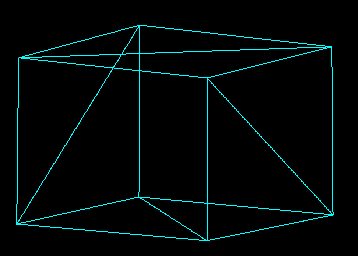
\includegraphics[width=\textwidth]{screenshot.png}
	\caption{A screenshot of the result.}
	\label{figure:outcome}
\end{figure}

% -----------------------------------------
\section{Classes and Mechanics}
\label{section:classes}

\subsection{Renderer} 

It is the class managing the meshes and the right application of the camera's and the meshes' matrices. It has got a Render method which goes through all meshes and converts their vertex coordinates to drawable screen coordinates.

The conversion calculations used are like shown in listing \ref{listing:conversion}.

\begin{lstlisting}[caption=The conversion from object coordinates to screen coordinates.,label=listing:conversion,language=C++]
// convert vertex from object coords to clip coords
mat4 modelViewProjectionMatrix = camera.projectionMatrix * 
	camera.viewMatrix * mesh->modelMatrix;

v = modelViewProjectionMatrix * v;

// normalize clip coordinates / get normalized device coordinates
v = v / v.w;

// clip vertices outside the viewport
if ((v.x < -1 || v.x > 1) ||
	(v.y < -1 || v.y > 1))
{
	// go to next vertex if this one is outside
	continue;
}

// map clip coordinates to screen coordinates
float width = screen->w;
float height = screen->h;
v.x = v.x * width * 0.5f + width * 0.5f;
v.y = -v.y * height * 0.5f + height * 0.5f;

vertex->screenPos = vec2(v.x, v.y);

drawPixel(vertex->screenPos, screen, 255, 0, 0);
\end{lstlisting}

\subsection{Camera} 

It creates the projection and the view matrix. The view matrix is constructed like in listing \ref{listing:viewmatrix}. The camera has a position, a target which it looks at and an up vector.

\begin{lstlisting}[caption=The View Matrix,label=listing:viewmatrix,language=C++]
vec3 f = normalize(target - position); // lookdirection vector
vec3 s = normalize(cross(f, up)); // orthogonal to layer defined by lookdirection and up
vec3 u = cross(s, f);

viewMatrix = mat4(
	s.x, u.x, -f.x, 0,
	s.y, u.y, -f.y, 0,
	s.z, u.z, -f.z, 0,
	-dot(s, position), -dot(u, position), dot(f, position), 1
	);
\end{lstlisting}

In the following listing (listing \ref{listing:perspectiveprojection}) the perspective projection matrix calculation is shown.

\begin{lstlisting}[caption=The Perspective Projection Matrix, label=listing:perspectiveprojection, language=C++]
float e = 1 / tan(frustum.fov * 0.5f);
float A = e / frustum.aspect;
float B = (-frustum.far - frustum.near) / (frustum.far - frustum.near);
float C = (-2 * frustum.far * frustum.near)/(frustum.far - frustum.near);


projectionMatrix = mat4(
	e, 0, 0, 0,
	0, A, 0, 0,
	0, 0, B, C,
	0, 0, -1, 0
	);
\end{lstlisting}

\subsection{Mesh}

A mesh contains a vector of vertices which store their positions. Meshes are represented as line loops. The vertices are drawn in the same order in which they are stored in the vector. When the end of the vector has been reached, the last vertex is connected to the first one. Meshes have a homogeneous model matrix describing the mesh's orientation, position and scale.

\newpage
\lstlistoflistings
\listoffigures

\end{document}